%%
%% This is file `Thesis.cls', based on 'ECSthesis.cls', by Steve R. Gunn
%% generated with the docstrip utility.
%%
%% Created by Steve R. Gunn, modified by Sunil Patel: www.sunilpatel.co.uk
\documentclass[11pt,letterpaper,notumble]{leaflet}
\usepackage[T1]{fontenc}
\usepackage[utf8]{inputenc}
\usepackage{listingsutf8}
\usepackage[spanish]{babel}
\usepackage{microtype}
\usepackage{blindtext} 
\usepackage{biolinum} 
\renewcommand\rmdefault{\sfdefault}% Verwende serifenlose Schrift 
\usepackage{mwe}% Dummy Bilder 
\usepackage{graphicx}
\usepackage{verbatim}
\usepackage{xcolor}
	\definecolor{WildStrawberry}{rgb}{1.0, 0.26, 0.64}
	\definecolor{wildstrawberry}{rgb}{1.0, 0.26, 0.64}
	\definecolor{Mulberry}{rgb}{0.77, 0.29, 0.55}
	\definecolor{LimeGreen}{rgb}{0.2, 0.8, 0.2}
	\definecolor{LincolnGreen}{rgb}{0.11, 0.35, 0.02}
	\definecolor{blue}{rgb}{0.0, 0.0, 1.0}
	\definecolor{forestgreen(traditional)}{rgb}{0.0, 0.27, 0.13}
\usepackage[colorlinks,citecolor=blue,urlcolor=blue]{hyperref}


\AddToBackground{5}{\put(0,0){\textcolor{blue!5}{\rule{\paperwidth}{\paperheight}}}}%

\AddToBackground{5}{% Fondo de la página pequeña 1
	\put(\LenToUnit{0.05\paperwidth},\LenToUnit{0.875\paperheight}){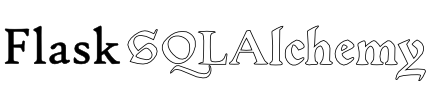
\includegraphics[width=\LenToUnit{0.90\paperwidth},height=\LenToUnit{0.1\paperheight}]{../img/flask-sqlalchemy-title.png}}
}

\title{Quik Reference} 
\author{Ferreira Juan David} 
\date{\today} % Experiment 1

\AddToBackground{1}{% Fondo de la página pequeña 1
	\put(\LenToUnit{0.05\paperwidth},\LenToUnit{0.7\paperheight}){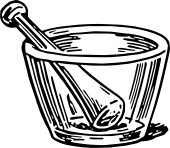
\includegraphics[width=\LenToUnit{0.70\paperwidth},height=\LenToUnit{0.25\paperheight}]{../img/flask-sqlalchemy-logo.png}}
}

%\AddToBackground{4}{\put(0,0){\textcolor{blue!5}{\rule{\paperwidth}{\paperheight}}}}%

\AddToBackground{1}{% Fondo de la página pequeña 1
	\put(\LenToUnit{0.75\paperwidth},\LenToUnit{0.95\paperheight}){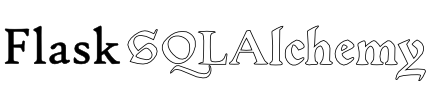
\includegraphics[width=\LenToUnit{0.90\paperwidth},height=\LenToUnit{0.1\paperheight},angle=270]{../img/flask-sqlalchemy-title.png}}
}



\begin{document}
	\mbox{}

	\vspace{16.5cm}
	
	\begin{tabular}{||c||c||c||}
		\hline
		\hline
		\rule[-1ex]{0pt}{2.5ex} id & username & email \\
		\hline
		\rule[-1ex]{0pt}{2.5ex} 1 & admin & admin@example.com \\
		\hline
		\rule[-1ex]{0pt}{2.5ex} 2 & peter & peter@example.org \\
		\hline
		\rule[-1ex]{0pt}{2.5ex} 3 & guest & guest@example.com \\
		\hline
		\hline
	\end{tabular}
	\thispagestyle{empty}% Keine Seitenzahlen 
	
	\clearpage
	\makebox[\linewidth][l]{
		\begin{minipage}{2.2\linewidth}
		    Recuperar un usuario por nombre de usuario:
		    
		    \lstset{inputencoding=utf8/latin1,
		    	frame=lines,
		    	label={lst:code_direct},
		    	basicstyle=\footnotesize,
		    	showstringspaces=false  
		    }
		    \lstinputlisting[language=Python,firstline=12,lastline=16]{../python/04-Select-Insert-Delete.py}
		    
		    Igual que el anterior, pero para un nombre de usuario no existente da \texttt{None}:
			
			\lstinputlisting[language=Python,firstline=18,lastline=20]{../python/04-Select-Insert-Delete.py}
			
			Seleccionar un grupo de usuarios mediante una expresión más compleja:
			
			\lstinputlisting[language=Python,firstline=22,lastline=23]{../python/04-Select-Insert-Delete.py}
			
			Ordenar usuarios por algo:
			
			\lstinputlisting[language=Python,firstline=25,lastline=26]{../python/04-Select-Insert-Delete.py}
			
			Limitar usuarios:
			
			\lstinputlisting[language=Python,firstline=28,lastline=29]{../python/04-Select-Insert-Delete.py}
			
			Obteniendo usuario por clave primaria:
			
			\lstinputlisting[language=Python,firstline=31,lastline=32]{../python/04-Select-Insert-Delete.py}
			
			\vspace*{-0.6cm}
			
			\section{Consultas en vistas}
			
			Si escribimos una función de vista de \texttt{Flask}, a menudo es muy útil devolver un error \texttt{404} para las vistas no definidas por el backend. Debido a que este es un idioma muy común, \texttt{Flask-SQLAlchemy} proporciona unos helpers para este propósito. En lugar de \texttt{get()} uno puede usar \texttt{get\_or\_404()} y en lugar de \texttt{first() first\_or\_404()}. Esto generará errores \texttt{404} en lugar de devolver \texttt{None}:
	
			\lstinputlisting[language=Python,firstline=34,lastline=37]{../python/04-Select-Insert-Delete.py}
			
			Además, si desea agregar una descripción con \texttt{abort()}, también puede usarla como argumento.
			
			\lstinputlisting[language=Python,firstline=39,lastline=39]{../python/04-Select-Insert-Delete.py}	
		\end{minipage}
		
	}
	\clearpage % end the column
	\mbox{}
	\clearpage
	
	\mbox{}
	
	\clearpage % end the spanned column
	
	\maketitle
	\begin{abstract}
		Ahora que ha declarado modelos , es hora de consultar los datos de la base de datos. Usaremos las definiciones de modelo del capítulo Inicio rápido.
	\end{abstract}

    \section{Insertar registros}
    
    Antes de que podamos consultar algo, tendremos que insertar algunos datos. Todos sus modelos deben tener un constructor, así que asegúrese de agregar uno si lo olvidó. Los constructores solo los usa usted, no \texttt{SQLAlchemy} internamente, por lo que depende completamente de usted cómo los defina.
    
    Insertar datos en la base de datos es un proceso de tres pasos:
    
    \begin{enumerate}
    	\item Crea el objeto \texttt{Python}.
    	
    	\item Agrégalo a la sesión.
    	
    	\item Comprometer la sesión.
    \end{enumerate}
    
    La sesión aquí no es la sesión de \texttt{Flask}, sino la de \texttt{Flask-SQLAlchemy}. Es esencialmente una versión reforzada de una transacción de base de datos. Así es como funciona:
    
    \lstset{inputencoding=utf8/latin1,
    	frame=lines,
    	label={lst:code_direct},
    	basicstyle=\footnotesize,
    	showstringspaces=false  
    }
    \lstinputlisting[language=Python,
    firstline=1,
    lastline=4]{../python/04-Select-Insert-Delete.py}
	
	\thispagestyle{empty}
	
	\clearpage
			
	    Muy bien, eso no fue difícil. ¿Qué pasa en qué momento? Antes de agregar el objeto a la sesión, \texttt{SQLAlchemy} básicamente no planea agregarlo a la transacción. Eso es bueno porque aún puede descartar los cambios. Por ejemplo, piense en crear la publicación en una página, pero solo desea pasar la publicación a la plantilla para obtener una vista previa en lugar de almacenarla en la base de datos.
			
	    La llamada a la función \texttt{add()} agrega el objeto. Emitirá una declaración \texttt{INSERT} para la base de datos, pero debido a que la transacción aún no está confirmada, no obtendrá una identificación de inmediato. Si realiza la confirmación, su usuario tendrá una \texttt{ID}:
			
	    \lstset{inputencoding=utf8/latin1,
	    	frame=lines,
	    	label={lst:code_direct},
	    	basicstyle=\footnotesize,
	    	showstringspaces=false  
	    }
	    \lstinputlisting[language=Python,firstline=6,lastline=7]{../python/04-Select-Insert-Delete.py}
			
	    \vspace*{-0.4cm}
		
		\section{Eliminar registros}
		    
		Eliminar registros es muy similar, en lugar de \texttt{add()} usar \texttt{delete()}:
		    
		\lstinputlisting[language=Python,firstline=9,lastline=10]{../python/04-Select-Insert-Delete.py}
		    
		\vspace*{-0.4cm}
		    
		\section{Consultando registros}
		    
		Entonces, ¿cómo recuperamos los datos de nuestra base de datos?. Para este propósito, \texttt{Flask-SQLAlchemy} proporciona un queryatributo en su clase \texttt{Model}. Cuando acceda, obtendrá un nuevo objeto de consulta sobre todos los registros. A continuación, puede utilizar métodos como \texttt{filter()} filtrar los registros antes de activar la selección con \texttt{all()} o \texttt{first()}. Si desea utilizar la clave principal, también puede utilizar \texttt{get()}.
		
		Las siguientes consultas asumen las siguientes entradas en la base de datos:
	
\end{document}